%% The first command in your LaTeX source must be the \documentclass command.
%%
\documentclass[jec]{acnsart}

% 允许更灵活的断行以避免 overfull hbox
\tolerance=1000
\emergencystretch=3em
\hfuzz=2pt
\sloppy

% 抑制部分无害警告
\usepackage{silence}
\usepackage{amsmath}
\usepackage{amssymb}
\usepackage{graphicx}
\usepackage{placeins}

% 让LaTeX更积极地放置浮动体
\renewcommand{\topfraction}{0.95}
\renewcommand{\bottomfraction}{0.95}
\renewcommand{\textfraction}{0.05}
\renewcommand{\floatpagefraction}{0.8}

% 减少图表与正文之间的间距
\setlength{\textfloatsep}{4pt plus 1pt minus 1pt}
\setlength{\floatsep}{4pt plus 1pt minus 1pt}
\setlength{\intextsep}{4pt plus 1pt minus 1pt}
\setlength{\abovecaptionskip}{3pt}
\setlength{\belowcaptionskip}{1pt}

\graphicspath{{./figures/}{figures/}{./}}
\WarningFilter{hyperref}{Ignoring empty anchor}
\WarningFilter{scrartcl}{Incompatible usage}
\WarningFilter{pdfx}{Setting all color commands}
\WarningFilter{doclicense}{The pdfx package was detected}
\WarningFilter{mathdesign}{No font specified}
\WarningFilter{mathdesign}{`bookman' option not defined}

\setdoi{10.55056/jec.ARTNUM}
\setjournalyear{2025}
\setjournalvolume{1}
\setjournalissue{1}
\setcounter{page}{1}


%%
%% end of the preamble, the start of the body of the document source.

%%
%% The "title" command
\title{Physics-Guided Contrastive Learning for Low-Latency On-Device Wearable Fall Detection}
\shorttitle{Physics-Guided Contrastive Learning for Edge Wearable Fall Detection}

%%
%% The "author" command and its associated commands are used to define
%% the authors and their affiliations.

% Authors and affiliations removed for anonymous review
\author[1]{Anonymous Author(s)}
\shortauthors{Anonymous Author(s)}
\address[1]{Anonymous Institution}

\begin{document}

%%
%% The abstract is a summary of the work to be presented in the
%% article.
\begin{abstract}
Wearable fall detection on edge devices must satisfy strict latency, memory, and energy constraints without sacrificing sensitivity. PhyCL-Net addresses this setting with a time-domain architecture built around a Physics-Guided Dynamic Kernel (PDK) and Jerk-aware Fall-Aware Attention (FAA), thereby avoiding spectral preprocessing overhead. Hierarchical dual-view contrastive regularization is used only during training, whereas deployment retains only the backbone. Under 12-fold LOSO evaluation on SisFall, PhyCL-Net achieves 98.21\% $\pm$ 0.10\% accuracy and 98.16\% $\pm$ 0.10\% Macro-F1 across five seeds with 1.049M parameters and 0.150979 GFLOPs. Under the reported single-thread CPU protocol, median latency is 125.99\,ms, corresponding to a 31.5\% reduction relative to the matched spectral baseline. At a TPR of 95\%, the corresponding FPR is 0.72\%; when FPR is fixed at 1\%, TPR decreases by 2.73 percentage points, making the accuracy--efficiency trade-off explicit.
\end{abstract}

%%
%% Keywords. The author(s) should pick words that accurately describe
%% the work being presented. Separate the keywords with commas.
\begin{keywords}
  Edge AI \sep
  Wearable Fall Detection \sep
  Physics-Inspired Deep Learning \sep
  Contrastive Learning \sep
  Real-Time Inference \sep
  Resource-Constrained Deployment
\end{keywords}

%%
%% This command processes the author affiliation and title
%% information and builds the first part of the formatted document.
\maketitle

\section{Introduction}

Falls remain a major source of injury-related morbidity among older adults and motivate continuous monitoring solutions that can operate outside supervised clinical environments~\cite{Bergen2016Falls}. Wearable inertial sensing is attractive in this setting because it is inexpensive, always available, and compatible with privacy-preserving on-device inference~\cite{Wu2015Wearable}. The central challenge, however, is not only to maximize classification accuracy, but to do so under tight latency, memory, and energy constraints while keeping false alarms low enough for practical use~\cite{Ramachandran2020Survey,mubashir2013survey,Cvach2012AlarmFatigue}.

Recent deep models have improved wearable activity recognition, including convolutional backbones, recurrent models, and Transformer variants~\cite{wang2019deep,he2016resnet,hochreiter1997lstm,Vaswani2017Attention,Zeng2023TransformersEffective}. In fall detection, hybrid CNN--RNN systems and other high-capacity architectures can achieve strong benchmark results~\cite{Liu2023FallEnsemble,Butt2022FallLSTM}, but they often increase runtime cost and are rarely analyzed from the perspective of deployment-oriented operating points. A second line of work improves discriminability through time--frequency representations such as STFT- or wavelet-based pipelines~\cite{Zhang2022TFC}. These representations can be effective, yet their preprocessing overhead is difficult to justify when low-latency inference is a primary design objective.

Despite this progress, three gaps remain. First, the literature still lacks a clear edge-oriented account of what is gained and lost when spectral preprocessing is removed under a matched implementation. Second, many existing models rely on generic temporal modules without exploiting fall-specific kinematic cues, even though falls are characterized by short impact transients and rapid jerk changes~\cite{Kim2024GaitPattern}. Third, contrastive objectives have improved time-series representation learning~\cite{chen2020simclr,Eldele2021TSTCC,Zhang2022TFC}, but they are usually discussed in terms of representation quality rather than whether they can regularize training without increasing inference cost.

These observations motivate a time-domain design that uses lightweight physical priors instead of an explicit spectral branch. We therefore propose PhyCL-Net, a physics-guided network for edge-oriented wearable fall detection. The model combines a Physics-Guided Dynamic Kernel (PDK), which adapts temporal receptive fields to local signal dynamics, with a Jerk-aware Fall-Aware Attention (FAA) module, which emphasizes transient segments that are more likely to correspond to fall impacts. A training-only hierarchical dual-view contrastive objective is added to improve feature separability, and its auxiliary heads are removed after training so that deployment cost is determined solely by the backbone.

Under 12-fold leave-one-subject-out (LOSO) evaluation on SisFall, PhyCL-Net achieves 98.21\%$\pm$0.10\% accuracy and 98.16\%$\pm$0.10\% Macro-F1 across five random seeds. The model uses 1.049M parameters and 0.150979 GFLOPs, and under the reported single-thread CPU protocol it reduces median latency from 184.31\,ms to 125.99\,ms relative to the matched spectral baseline. At the operating point TPR${=}$95\%, the corresponding FPR is 0.72\%; when FPR is constrained to 1\%, TPR decreases by 2.73 percentage points relative to the spectral variant. These results quantify the accuracy--efficiency trade-off rather than assuming it.

The main contributions of this work are as follows:
\begin{itemize}
\item We present an edge-oriented comparison between a physics-guided time-domain backbone and a matched spectral baseline under a common implementation and benchmarking protocol.
\item We introduce PDK and FAA as lightweight modules that encode fall-relevant kinematic priors without adding a frequency-domain branch.
\item We use hierarchical dual-view contrastive regularization only during training, improving representation quality while keeping inference-time cost unchanged.
\item We report deployment-relevant operating points, including FPR@TPR${=}$95\% and TPR@FPR${=}$1\%, in addition to headline classification metrics.
\end{itemize}

\section{Proposed Method}

This section defines the learning problem, summarizes the overall architecture, and then explains the rationale behind each component. The task is formulated as window-based binary time-series classification: each sample $(X_i, y_i)$ contains an inertial window $X_i \in \mathbb{R}^{C \times T}$ and a label $y_i \in \{0,1\}$, where $1$ denotes a fall and $0$ denotes an activity of daily living. Training minimizes class-weighted cross-entropy together with the training-only contrastive regularizer introduced in Section~2.5.

\FloatBarrier
\subsection{Overview of PhyCL-Net}
PhyCL-Net is a compact time-domain backbone consisting of a lightweight stem followed by three stages that progressively reduce temporal resolution. For input $X \in \mathbb{R}^{B \times 3 \times 512}$, the stem applies GhostConv1d ($k{=}5, s{=}1, p{=}2$), mapping 3 channels to 48 while preserving $T{=}512$. Stage~1 operates at $(C,T){=}(48,512)$ with two PhyCL-Blocks. Transition layers use SeparableConv1d ($k{=}5, s{=}2, p{=}2$) for downsampling, so Stage~2 operates at $(96,256)$ and Stage~3 at $(192,128)$, again with two PhyCL-Blocks each. The classifier head uses AdaptiveAvgPool1d(1) followed by a linear layer from 192 to 2 logits.

The architecture is designed around two constraints. First, it must preserve the short transients that distinguish falls from vigorous activities of daily living. Second, it must do so with a compact computation graph suitable for edge-oriented benchmarking. Each PhyCL-Block therefore contains two complementary streams: PDK models multi-scale temporal context, whereas FAA highlights high-jerk intervals that are more likely to contain impact evidence. Their outputs are merged by a symmetric cross-gated fusion unit with residual scaling. Figure~\ref{fig:architecture} summarizes the full network and the internal structure of a PhyCL-Block.

\begin{figure}[!htbp]
\centering
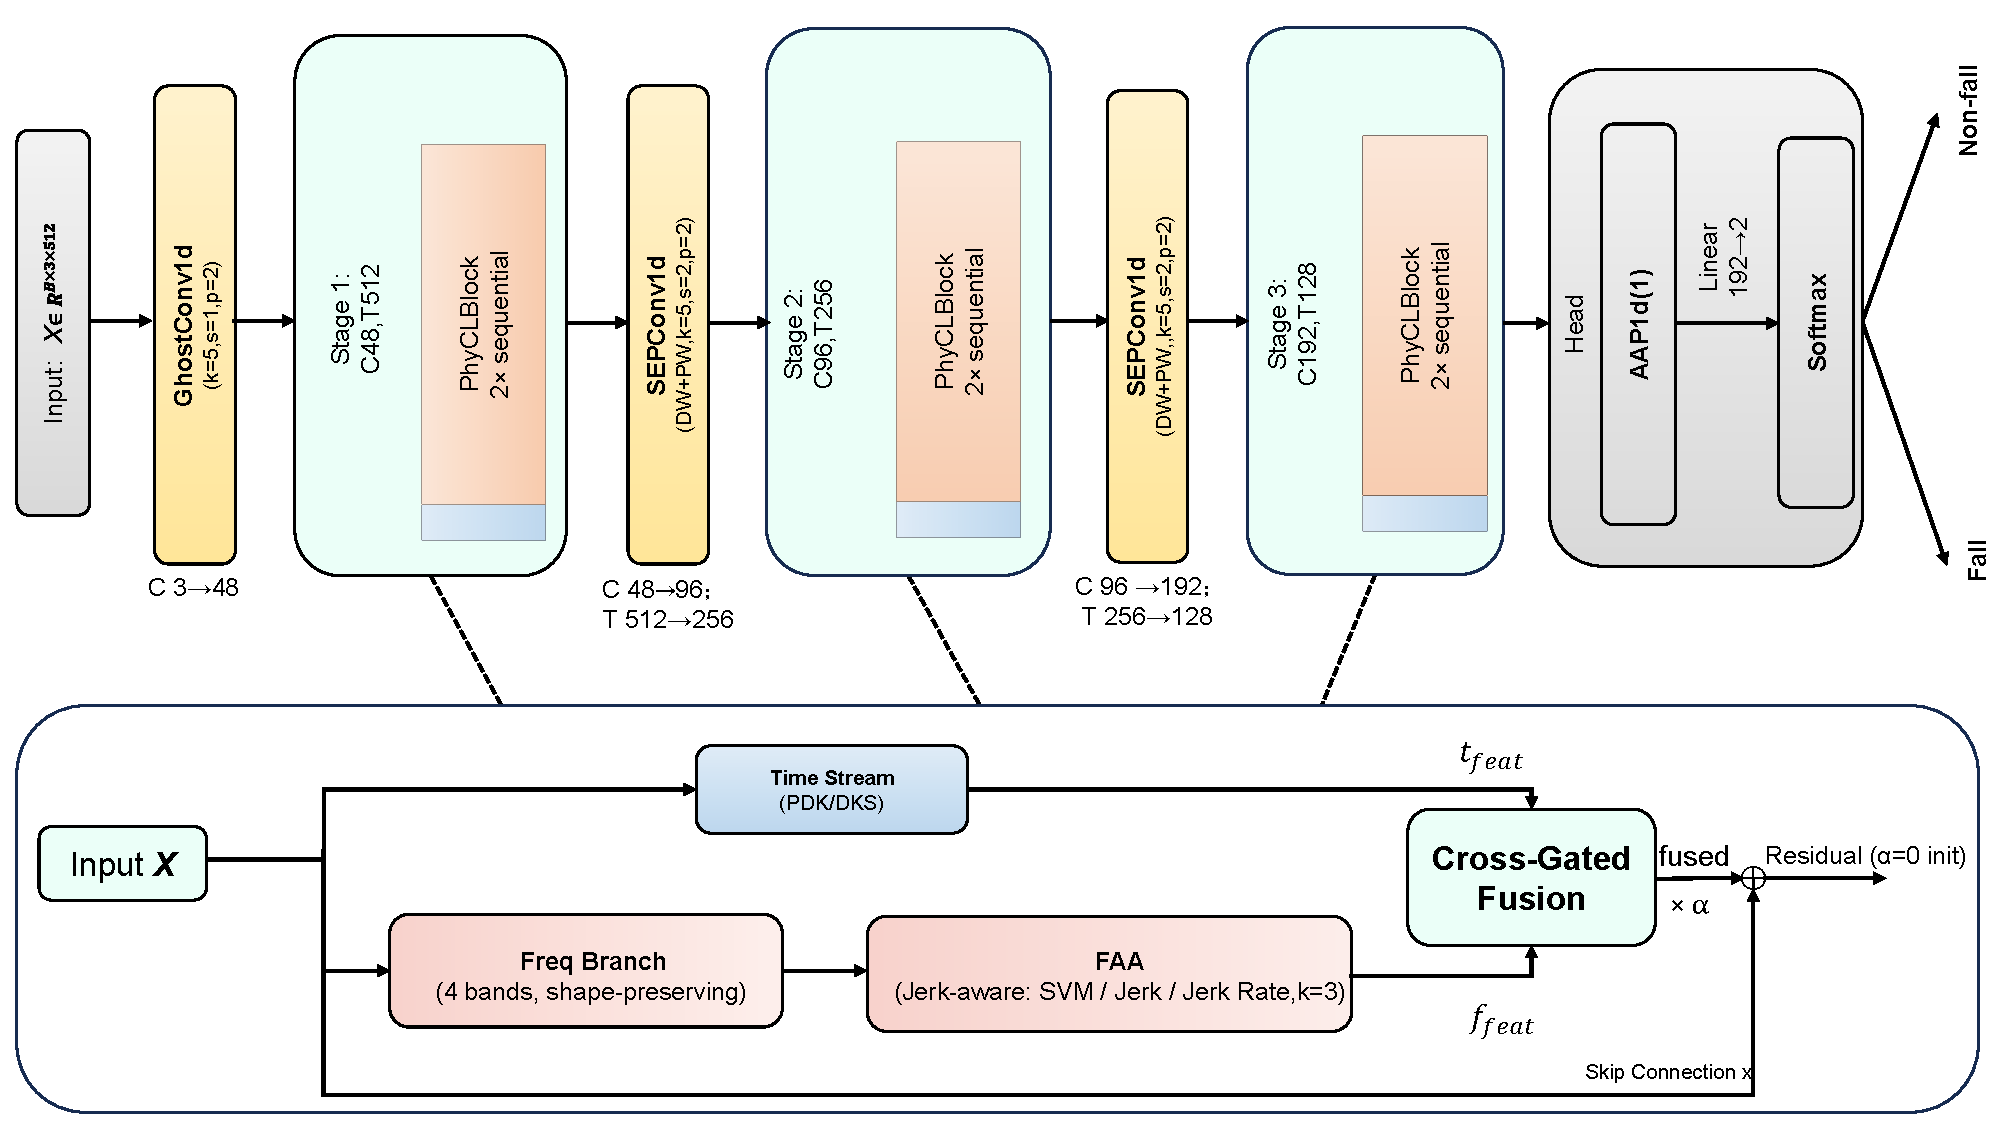
\includegraphics[width=0.85\linewidth]{figures/fig01_architecture_and_block.pdf}
\caption{The overall architecture of PhyCL-Net. The input signal is processed by two parallel branches: the Physics-Guided Dynamic Kernel (PDK) for adaptive receptive fields and the Fall-Aware Attention (FAA) for jerk extraction, fused via the Cross-Gated Fusion Unit. The detailed internal structure of a single PhyCL-Block is also shown, illustrating the two parallel streams (PDK for multi-scale temporal adaptation and FAA for transient emphasis) and their integration through the symmetric cross-gated fusion unit.}
\label{fig:architecture}
\end{figure}

\FloatBarrier

\subsection{Physics-Guided Dynamic Kernel (PDK)}
Falls exhibit mixed temporal dynamics: a short, high-energy impact is often followed by a slower transition phase~\cite{Kim2024GaitPattern}. A single fixed kernel therefore risks missing either the transient or the broader temporal context. PDK addresses this mismatch by routing features through a small set of depthwise 1D kernels with sizes $\{7,15,31,63\}$, chosen to cover short, medium, and long temporal patterns while keeping the candidate set small enough for efficient execution. Inspired by selective kernel networks~\cite{li2019sknet}, the module then forms an input-dependent mixture over these branches.

The routing weights are predicted from two lightweight signals: (i) a 12-dimensional physics descriptor $p=\phi(X)\in\mathbb{R}^{12}$ extracted from the input window, containing support vector magnitude, jerk, jerk rate, and related transient cues, and (ii) a 4-way complexity logit $\ell^{\mathrm{cmp}}$ derived from globally pooled features. A three-layer physics MLP ($12{\rightarrow}32{\rightarrow}32{\rightarrow}4$) maps $p$ to $w^{\mathrm{phy}}\in\mathbb{R}^{4}$, while a two-layer complexity MLP ($C{\rightarrow}32{\rightarrow}4$) produces $\ell^{\mathrm{cmp}}$. Their element-wise product is normalized using a learnable softmax temperature $\tau_{\mathrm{dks}}=\max(0.1,\tilde{\tau}_{\mathrm{dks}})$, initialized to 1.0, yielding the routing weights $a=\mathrm{Softmax}((\ell^{\mathrm{cmp}}\odot w^{\mathrm{phy}})/\tau_{\mathrm{dks}})$. The PDK output is
\begin{equation}
\label{eq:pdk}
\mathrm{PDK}(F) = \sum_{k\in\mathcal{K}} a_k\, \mathrm{DWConv}_{k}(F), \quad \mathcal{K}=\{7,15,31,63\},
\end{equation}
where $\mathrm{DWConv}_{k}$ denotes depthwise 1D convolution with kernel size $k$, $\mathrm{GAP}(\cdot)$ is AdaptiveAvgPool1d(1), and $\odot$ denotes element-wise multiplication. The resulting module remains a single-pass time-domain operator and avoids explicit time--frequency transforms. Figure~\ref{fig:pdk_module} shows the detailed PDK structure.

\begin{figure}[!htbp]
\centering
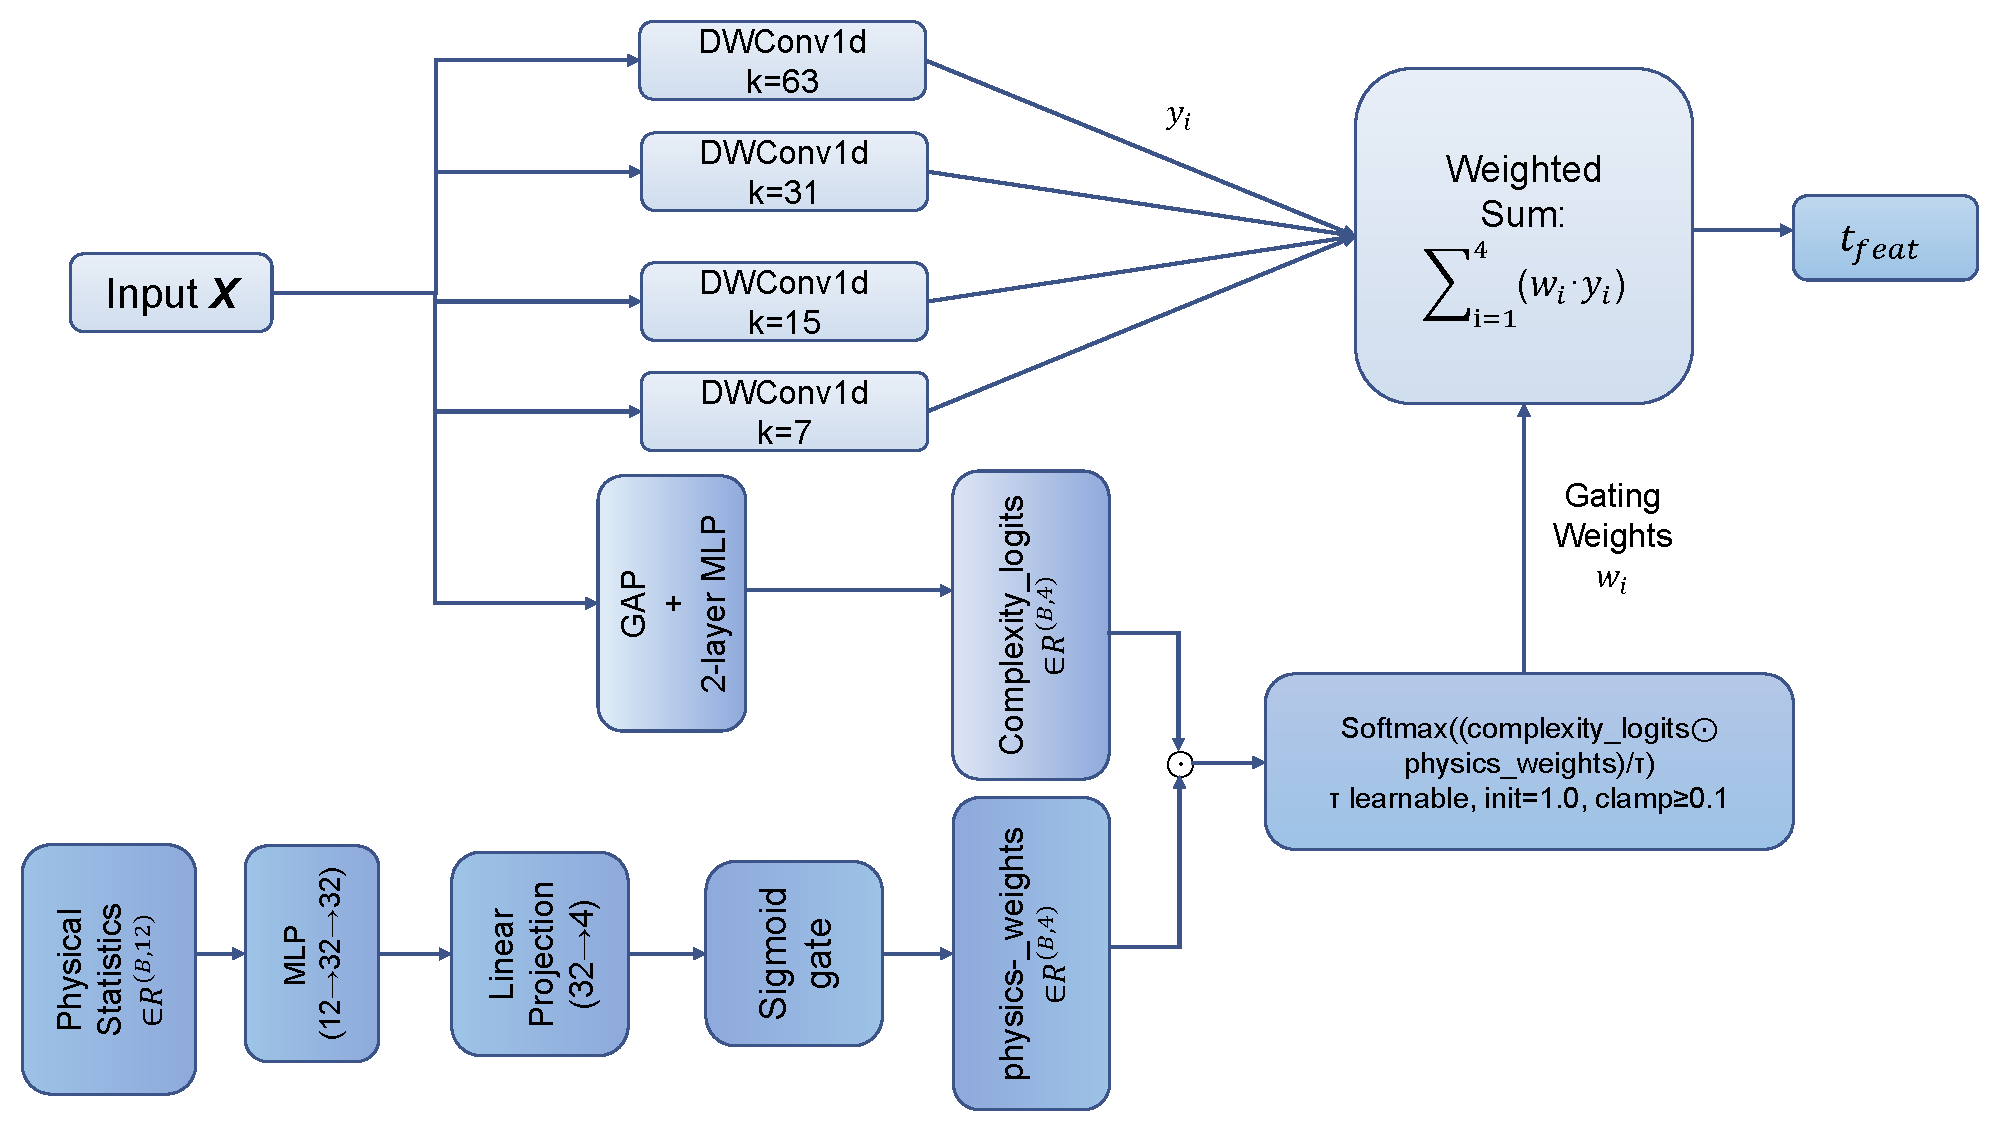
\includegraphics[width=0.85\linewidth]{figures/fig02_pdk_module.pdf}
\caption{Physics-Guided Dynamic Kernel (PDK) module with Dynamic Kernel Selection (DKS). The module routes features through multiple temporal kernels with input-dependent mixture weights derived from physics descriptors.}
\label{fig:pdk_module}
\end{figure}

\subsection{Jerk-aware Fall-Aware Attention (FAA)}
A common failure mode in fall detection is confusion between falls and vigorous activities of daily living~\cite{Zafar2025FallTransformer}. FAA introduces a kinematics-aligned bias by emphasizing jerk-dominant segments, where rapid temporal change is more likely to coincide with an impact. To keep the module lightweight, the attention mask is generated by a depthwise temporal operator followed by normalization and pointwise nonlinearity:
\begin{equation}
\label{eq:faa}
M = \sigma\bigl(\mathrm{GELU}(\mathrm{GN}(\mathrm{DWConv}_{3}(F)))\bigr), \qquad
\mathrm{FAA}(F) = F \odot M + F,
\end{equation}
where $\mathrm{GN}(\cdot)$ denotes GroupNorm, $\odot$ denotes element-wise multiplication, and $\sigma$ is the sigmoid function. The residual form preserves the original feature stream and makes FAA an inductive bias rather than a hard filter.

\subsection{Symmetric Cross-Gated Fusion}
\label{sec:fusion}
PDK and FAA provide complementary evidence: PDK captures multi-scale temporal context, whereas FAA emphasizes transient saliency~\cite{hou2021coordinate}. A direct concatenation would increase channel dimensionality and defer the interaction between both streams to later layers. Instead, we use a symmetric cross-gated unit so that each stream can modulate the other before fusion. Let $t=\mathrm{PDK}(F)$ and $f=\mathrm{FAA}(F)$. Multi-scale channel gates with kernels $r\in\{3,5,7\}$ are defined as $g_t = \sigma(\sum_{r} \mathrm{Conv}^{\mathrm{ch}}_{r}(\mathrm{GAP}(f)))$ and $g_f = \sigma(\sum_{r} \mathrm{Conv}^{\mathrm{ch}}_{r}(\mathrm{GAP}(t)))$. The gated representation $\tilde{F} = t \odot g_t + f \odot g_f$ is then refined by spatial attention $a_s = \sigma(\mathrm{Conv}^{\mathrm{sp}}_{7}([\mathrm{AvgPool}(\tilde{F});\mathrm{MaxPool}(\tilde{F})]))$. The final output is
\begin{equation}
\label{eq:fusion}
F_{\mathrm{out}} = F + \alpha\,(\tilde{F} \odot a_s),
\end{equation}
where $\mathrm{Conv}^{\mathrm{ch}}_{r}$ denotes a channel-gating operator with kernel size $r$, $\mathrm{Conv}^{\mathrm{sp}}_{7}$ denotes a spatial attention convolution with kernel size 7, and the residual scaling $\alpha$ is learnable and initialized to 0.0. Figure~\ref{fig:cross_gate_fusion} illustrates the fusion unit.

\begin{figure}[!htbp]
\centering
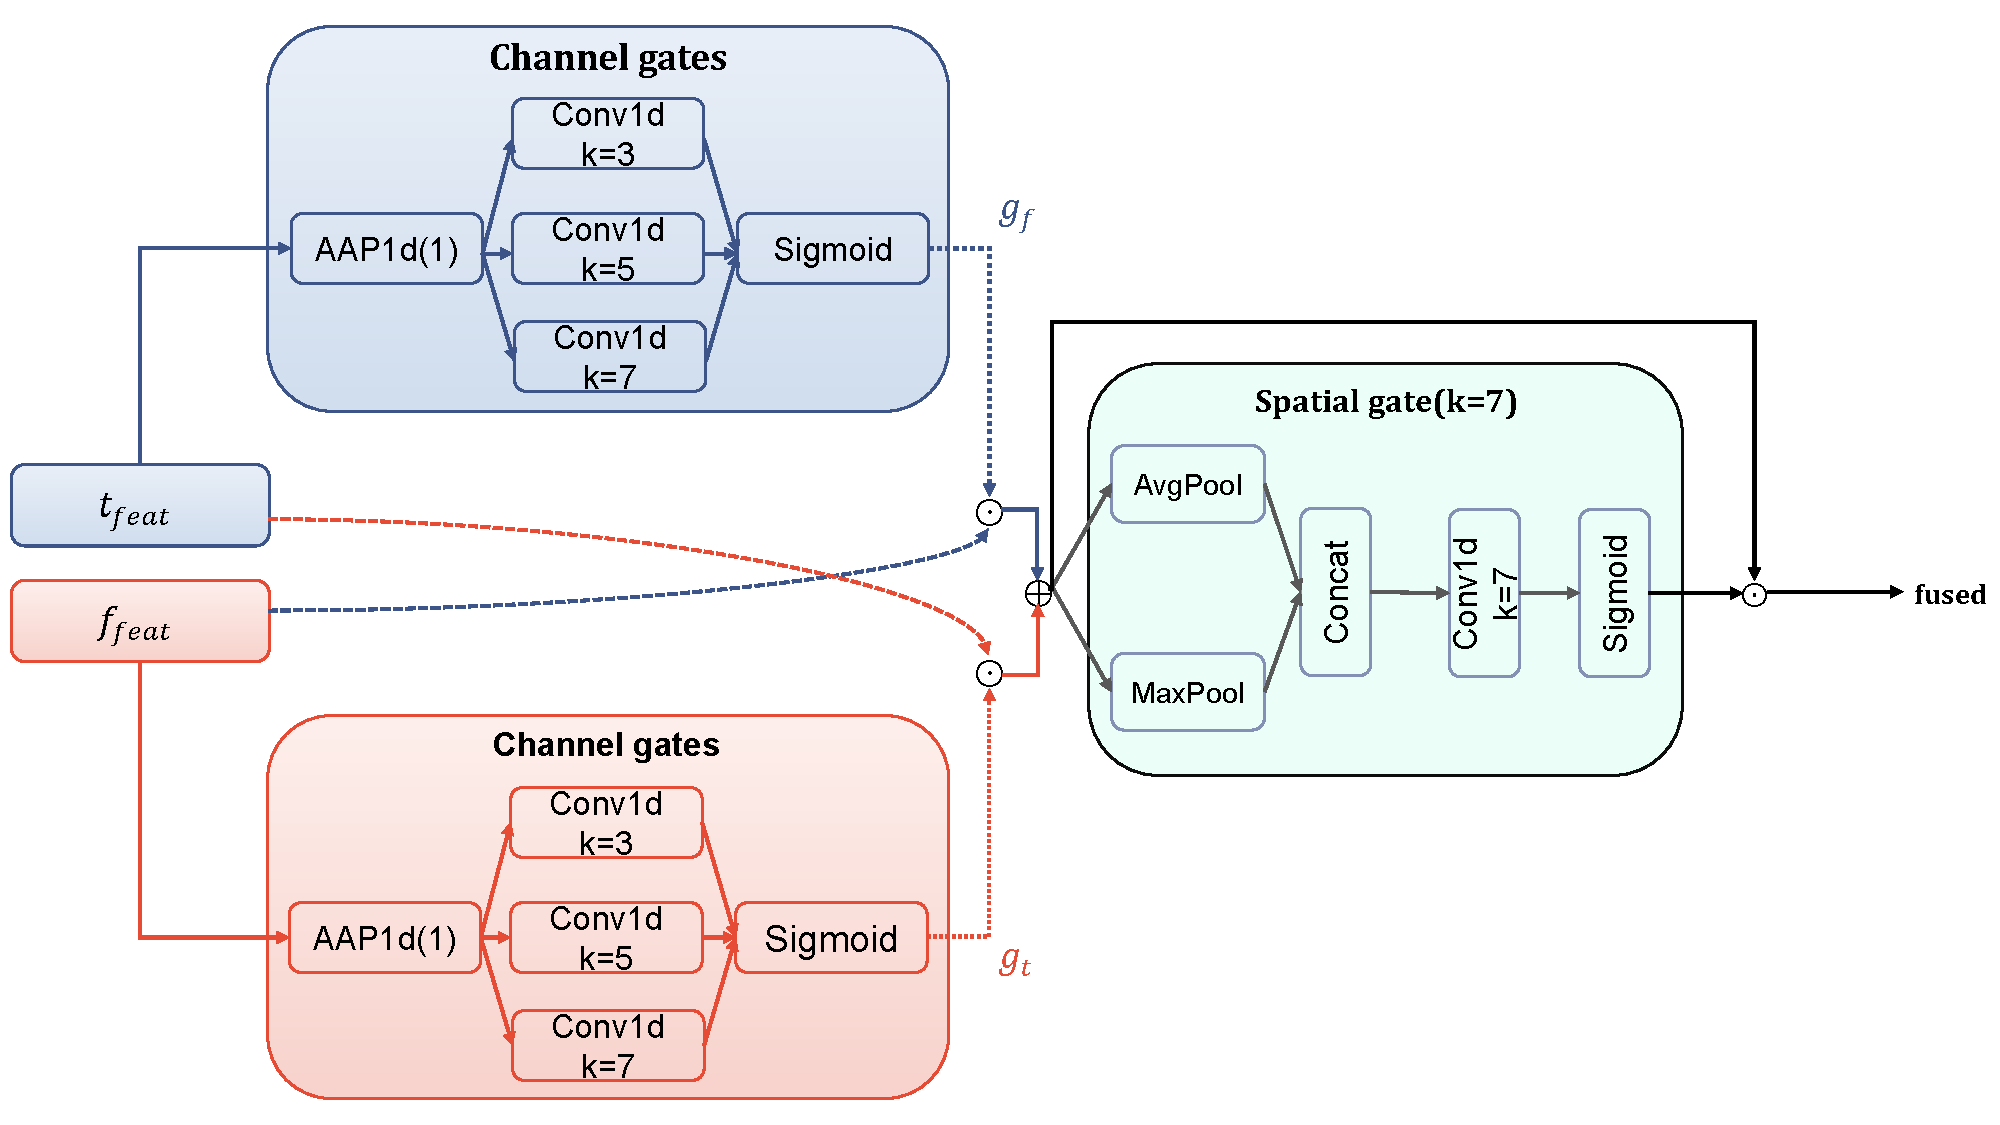
\includegraphics[width=0.85\linewidth]{figures/fig03_cross_gate_fusion.pdf}
\caption{Symmetric Cross-Gated Fusion Unit. Each stream modulates the other through multi-scale channel gating and spatial attention, producing a unified representation that combines multi-scale temporal context from PDK with transient saliency from FAA.}
\label{fig:cross_gate_fusion}
\end{figure}

\subsection{Training-only Hierarchical Dual-view Contrastive Regularization}
To enhance feature separability without increasing deployment cost, we introduce a training-only contrastive regularizer based on the InfoNCE objective~\cite{chen2020simclr,Zhang2022TFC}. Six auxiliary projection heads (three stages $\times$ two streams) are attached during training, each consisting of global average pooling followed by a linear projection to 128 dimensions. The heads are discarded after training, so the deployed model is identical to the backbone used for standard inference.

Given a batch of $N$ input windows, we apply two independent stochastic augmentations $t_1(\cdot)$ and $t_2(\cdot)$~\cite{Iwana2021DataAugmentation} to generate paired views. For each sample $X_i$, the backbone $f_\theta$ and projection head $h$ produce $\ell_2$-normalized embeddings:
\begin{equation}
\label{eq:tfcl_embed}
z_i^{(q)}=\frac{h(f_\theta(t_q(X_i)))}{\|h(f_\theta(t_q(X_i)))\|_2}, \quad q\in\{1,2\}.
\end{equation}
The contrastive loss encourages embeddings from the same sample to align while separating those from different samples. We adopt a symmetric InfoNCE formulation with cosine similarity $\mathrm{sim}(u,v) = u^\top v$ and temperature $\tau = 0.1$:
\begin{equation}
\label{eq:tfcl_infonce}
\mathcal{L}_{\mathrm{NCE}} = -\frac{1}{2N}\sum_{i=1}^{N}\bigl[\ell_i^{(1\to2)} + \ell_i^{(2\to1)}\bigr],
\end{equation}
where $\ell_i^{(q\to q')}$ denotes the log-softmax probability of correctly identifying the positive pair among all negatives in the batch. The final training objective combines the classification loss with the contrastive term:
\begin{equation}
\label{eq:tfcl_total}
\mathcal{L} = \mathcal{L}_{\mathrm{CE}}+\lambda_{\mathrm{tfcl}}\,\mathcal{L}_{\mathrm{NCE}}, \quad \lambda_{\mathrm{tfcl}}= 0.1.
\end{equation}

\subsection{Reproducibility and Deployment Protocol}
To improve traceability, PhyCL-Net and the spectral baseline share the same codebase and differ only by a configuration switch that enables or removes the spectral branch. Each run exports structured outputs including aggregated metrics, fold-level LOSO results, efficiency measurements, and training logs. This organization allows direct auditing of both accuracy and efficiency results.

For static complexity, FLOPs and parameter counts are computed with forced CPU execution at input shape $1 \times 3 \times 512$. For runtime performance, latency is measured on the CPU in single-thread mode and reported as p50/p95 at batch sizes 1 and 32, together with the software environment. The release materials described in the data availability statement include the configuration files and machine-readable artifacts required to reproduce the reported measurements.


\section{Experimental Setup and Results}

This section first describes the dataset, preprocessing pipeline, evaluation protocol, and training setup, and then reports the main results, efficiency measurements, operating-point analysis, and ablations. The goal is to separate what is supported directly by the present experiments from broader deployment claims that still require additional validation.

\subsection{Dataset and Preprocessing}

Evaluation is conducted on the SisFall benchmark using the widely adopted 12-subject subset (SA01, SA02, SA04, SA05, SA06, SA09, SA10, SA11, SA17, SA18, SA19, SA21) to reflect subject-independent deployment. The raw inertial streams are sampled at 200\,Hz and processed through a fixed pipeline: downsampling to 50\,Hz, 4th-order Butterworth low-pass filtering (5\,Hz cutoff), sliding-window segmentation with a window length of 512 and a stride of 256 (50\% overlap), per-channel z-score normalization, and zero-padding for windows shorter than 512. Unless otherwise specified, the 3-axis accelerometer channels (``accel3'') are used. The resulting evaluation set contains 21,678 windows (12,678 ADL and 9,000 FALL).

\subsection{Evaluation Protocol and Metrics}

We adopt a 12-fold leave-one-subject-out (LOSO) cross-validation scheme. To avoid reporting a favorable single training trajectory, we repeat PhyCL-Net with five random seeds (42, 123, 456, 789, 1024) and report the mean/standard deviation, along with 95\% confidence intervals.

Standard classification metrics assess performance. Accuracy is defined as
\begin{equation}
\label{eq:accuracy}
\mathrm{Accuracy} = \frac{\mathrm{TP} + \mathrm{TN}}{\mathrm{TP} + \mathrm{TN} + \mathrm{FP} + \mathrm{FN}}.
\end{equation}

Sensitivity, or true positive rate (TPR), is
\begin{equation}
\label{eq:sensitivity}
\mathrm{Sensitivity} = \frac{\mathrm{TP}}{\mathrm{TP} + \mathrm{FN}}.
\end{equation}

Specificity, or true negative rate (TNR), is
\begin{equation}
\label{eq:specificity}
\mathrm{Specificity} = \frac{\mathrm{TN}}{\mathrm{TN} + \mathrm{FP}}.
\end{equation}

G-Mean summarizes the balance between sensitivity and specificity:
\begin{equation}
\label{eq:gmean}
\mathrm{G\text{-}Mean} = \sqrt{\mathrm{TPR} \times \mathrm{TNR}}.
\end{equation}

Macro-F1 is the unweighted mean of the per-class F1 scores. Because continuous monitoring is constrained by false alarms~\cite{Cvach2012AlarmFatigue}, we also report operating-point metrics that explicitly control the false-positive rate. These quantities are recomputed on the LOSO test partitions and are used later to quantify the trade-off between false-alarm control and sensitivity.

\subsection{Training Setup}

Unless stated otherwise, we use a fixed training pipeline for SisFall LOSO. For the reported multi-seed setting, we train for 50 epochs with a batch size of 256, an initial learning rate of 0.004, and 10 warmup epochs. We use AdamW with weight decay $1{\times}10^{-4}$ and a CosineAnnealingLR schedule ($\eta_{\min}{=}1{\times}10^{-6}$). Mixed precision (AMP) is enabled, and gradients are clipped to a max norm of 1.0. The total loss is CE (weight 1.0) plus TFCL (weight 0.1) when enabled, with automatic inverse-frequency class weighting.

\begin{table}[htbp]
\caption{Training hyperparameters for the reported SisFall LOSO experiments.}
\label{tab:train_setup}
\centering
\small
\setlength{\tabcolsep}{4pt}
\begin{tabular}{lc}
\toprule
Setting & Value \\
\midrule
Optimizer & AdamW \\
Initial learning rate & 0.004 \\
Epochs & 50 \\
Warmup epochs & 10 \\
Batch size & 256 \\
Weight decay & $1{\times}10^{-4}$ \\
Scheduler & CosineAnnealingLR ($\eta_{\min}{=}1{\times}10^{-6}$) \\
AMP & True \\
Gradient clipping & 1.0 \\
Loss weights & CE: 1.0, TFCL: 0.1 \\
Class weighting & Auto (inverse frequency) \\
\bottomrule
\end{tabular}
\end{table}

\subsection{Baselines}

We compare our approach against representative time-series architectures commonly used in wearable sensing, including InceptionTime~\cite{fawaz2020inceptiontime}, a Temporal Convolutional Network (TCN), a lightweight Transformer variant~\cite{Vaswani2017Attention,Zeng2023TransformersEffective}, ResNet~\cite{he2016resnet}, and LSTM~\cite{hochreiter1997lstm}. Recent works have also explored ensemble CNN-RNN hybrids for fall detection~\cite{Liu2023FallEnsemble,Butt2022FallLSTM}. We also include the frequency-heavy in-house baseline MSPA-FAA-PDK, which retains the spectral branch, to isolate the accuracy--efficiency effect of removing spectral processing under an otherwise matched implementation.

\subsection{Main Results (LOSO on SisFall)}

Under LOSO, PhyCL-Net achieves 98.20\% Accuracy and 98.15\% Macro-F1, outperforming TCN (97.13\% Accuracy) and the Transformer baseline (95.48\% Accuracy). Across five seeds, performance remains stable at 98.21\%$\pm$0.10\% Accuracy and 98.16\%$\pm$0.10\% Macro-F1. Table~\ref{tab:main_results} summarizes the LOSO performance. Figure~\ref{fig:pareto_tradeoff} visualizes the accuracy--efficiency trade-off, where bubble size is proportional to CPU latency, demonstrating that PhyCL-Net achieves the best accuracy while maintaining competitive efficiency.

\begin{figure}[!htbp]
\centering
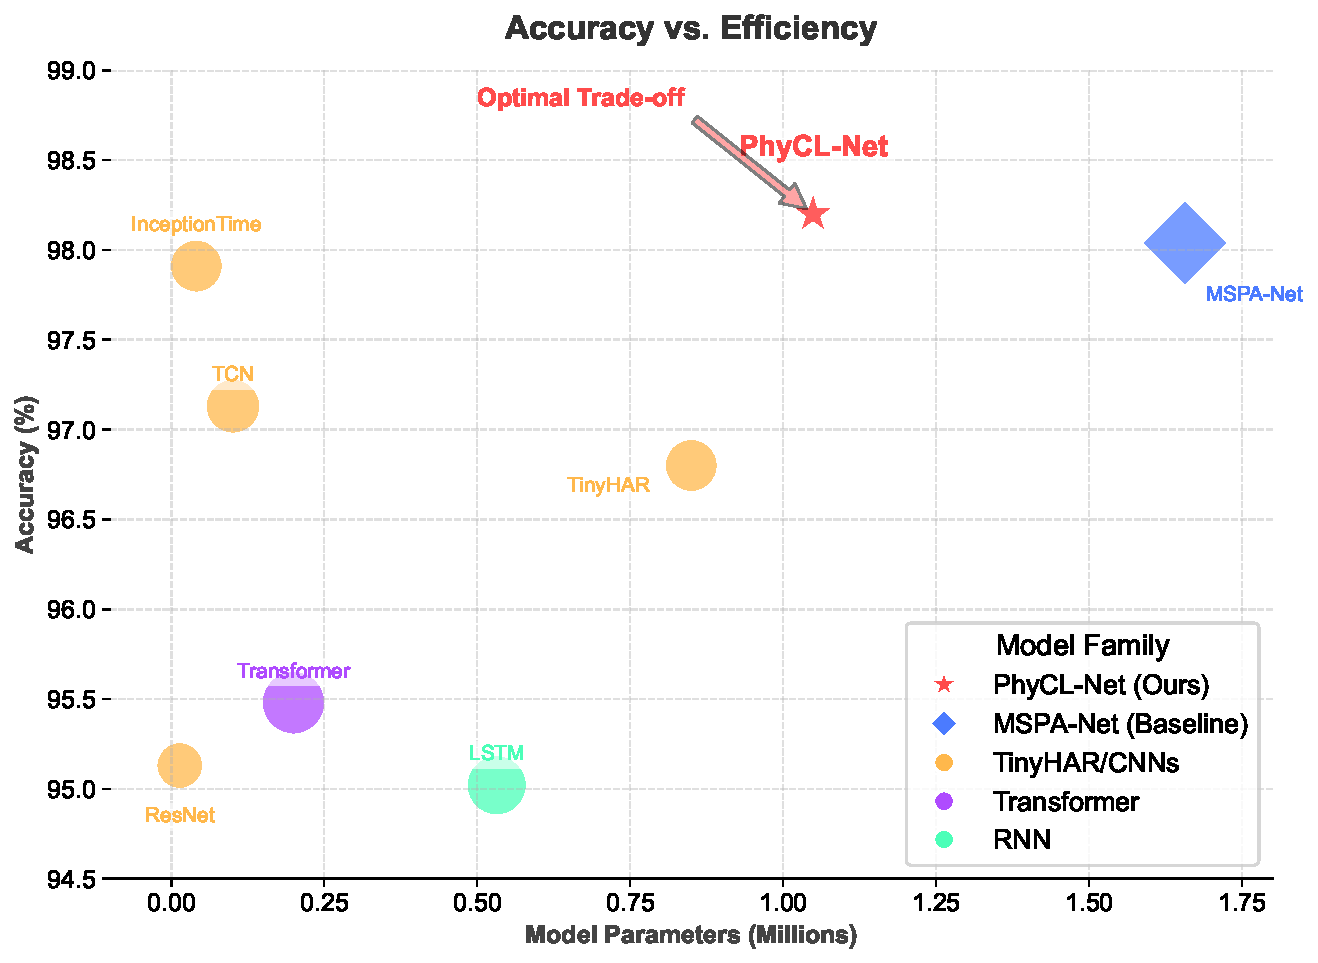
\includegraphics[width=0.85\linewidth]{figures/fig04_pareto_tradeoff.pdf}
\caption{Accuracy--efficiency trade-off. Bubble size is proportional to single-thread CPU latency (p50). PhyCL-Net (red star) achieves the best accuracy (98.20\%) while maintaining a competitive parameter count (1.049M) and low latency (125.99\,ms).}
\label{fig:pareto_tradeoff}
\end{figure}

\begin{table}[htbp]
\caption{LOSO performance on SisFall (12 folds). PhyCL-Net values are mean (95\% CI) aggregated across 5 random seeds; other models use 2 seeds with fold-level 95\% CI.}
\label{tab:main_results}
\centering
\footnotesize
\setlength{\tabcolsep}{4pt}
\begin{tabular}{@{}lccccc@{}}
\toprule
Model & Params & Acc (\%) & F1 (\%) & Sens (\%) & Spec (\%) \\
\midrule
\textbf{PhyCL-Net (ours)} & \textbf{1.049M} & \textbf{98.21} & \textbf{98.16} & \textbf{97.93} & \textbf{98.41} \\
 & & {\scriptsize(98.09--98.33)} & {\scriptsize(98.04--98.28)} & {\scriptsize(97.80--98.06)} & {\scriptsize(98.27--98.55)} \\
\midrule
MSPA-FAA-PDK & 1.657M & 98.04 & 97.98 & 97.67 & 98.30 \\
\midrule
InceptionTime & 0.041M & 97.91 & 97.85 & 97.82 & 97.97 \\
\midrule
TCN & 0.101M & 97.13 & 97.04 & 96.43 & 97.63 \\
\midrule
Transformer & 0.200M & 95.48 & 95.34 & 94.71 & 96.02 \\
\midrule
ResNet & 0.014M & 95.13 & 94.98 & 94.41 & 95.64 \\
\midrule
LSTM & 0.532M & 95.02 & 94.86 & 94.35 & 95.50 \\
\bottomrule
\end{tabular}
\end{table}

Figure~\ref{fig:fold_stability} presents the cross-validation stability analysis, displaying the fold-wise performance comparison across 12 subjects. The results indicate that PhyCL-Net consistently outperforms the baseline in nearly every fold, exhibiting lower variance and greater stability across subjects.

\begin{figure}[!htbp]
\centering
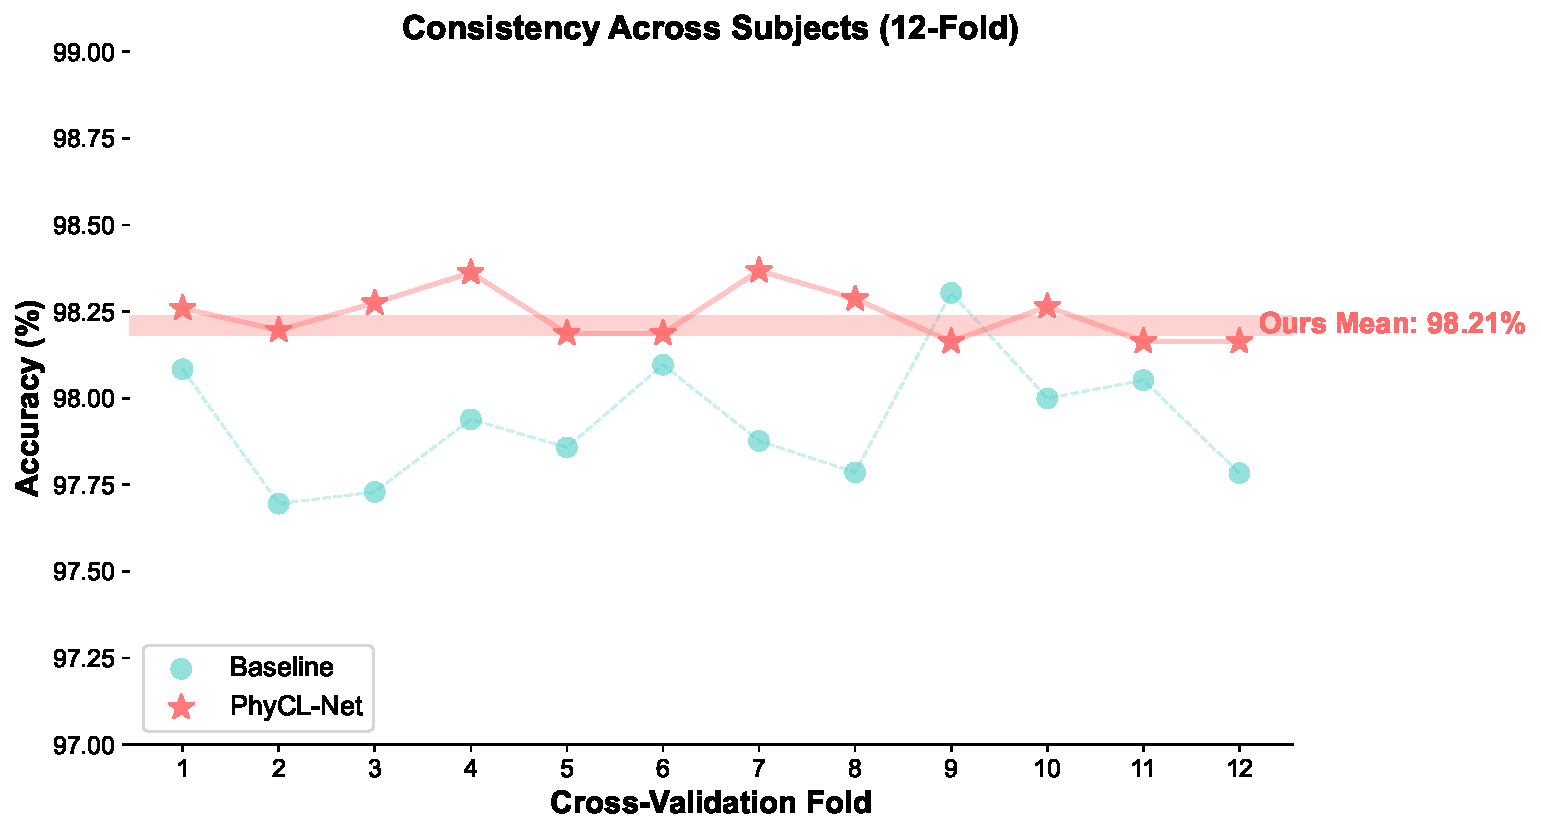
\includegraphics[width=0.85\linewidth]{figures/fig05_fold_stability.pdf}
\caption{Cross-validation stability analysis. The fold-wise comparison across 12 subjects shows that PhyCL-Net outperforms the matched spectral baseline in most folds and exhibits lower variance across subjects.}
\label{fig:fold_stability}
\end{figure}

Figures~\ref{fig:radar}--\ref{fig:confusion} provide complementary qualitative views of the results. The radar chart summarizes the multi-metric trade-off among the strongest models. The t-SNE projection illustrates class separation in the learned feature space. The FAA visualization highlights the temporal regions emphasized around impact-like transients. The confusion matrix shows that both classes are recognized with high recall. Recent graph-based time-series models~\cite{Jin2024GNNTimeSeries} suggest one possible future direction for modeling inter-channel dependencies, but such extensions are outside the scope of the present study.

\begin{figure}[!htbp]
\centering
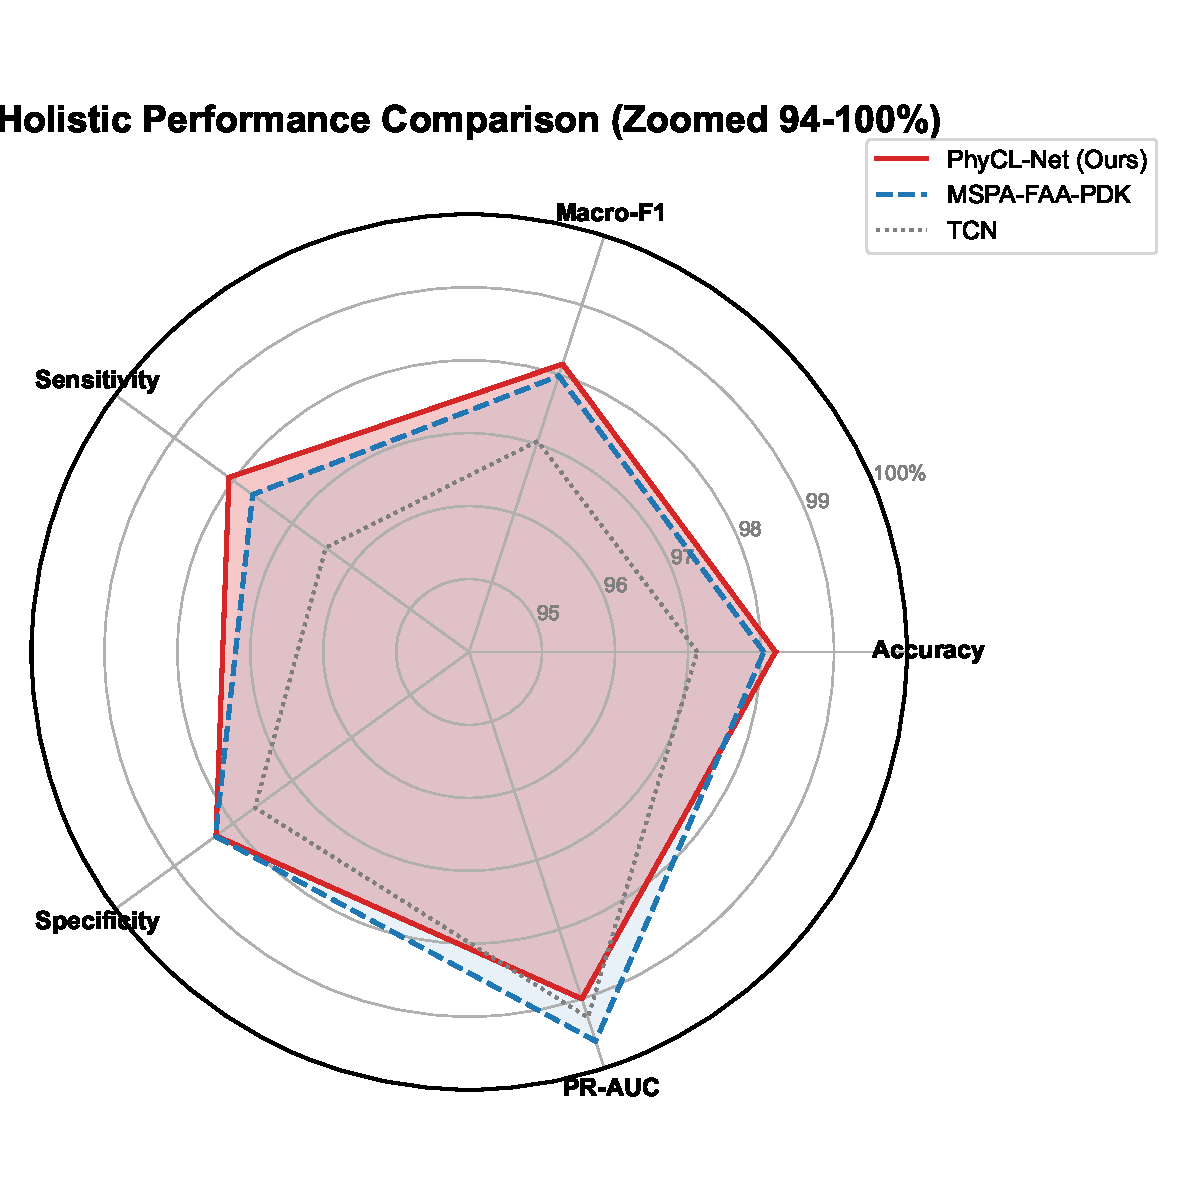
\includegraphics[width=0.75\linewidth]{figures/fig06_radar.pdf}
\caption{Radar chart comparing PhyCL-Net, MSPA-FAA-PDK, and TCN across four metrics. Axes are scaled from 95\% to 100\% to highlight differences.}
\label{fig:radar}
\end{figure}

\begin{figure}[!htbp]
\centering
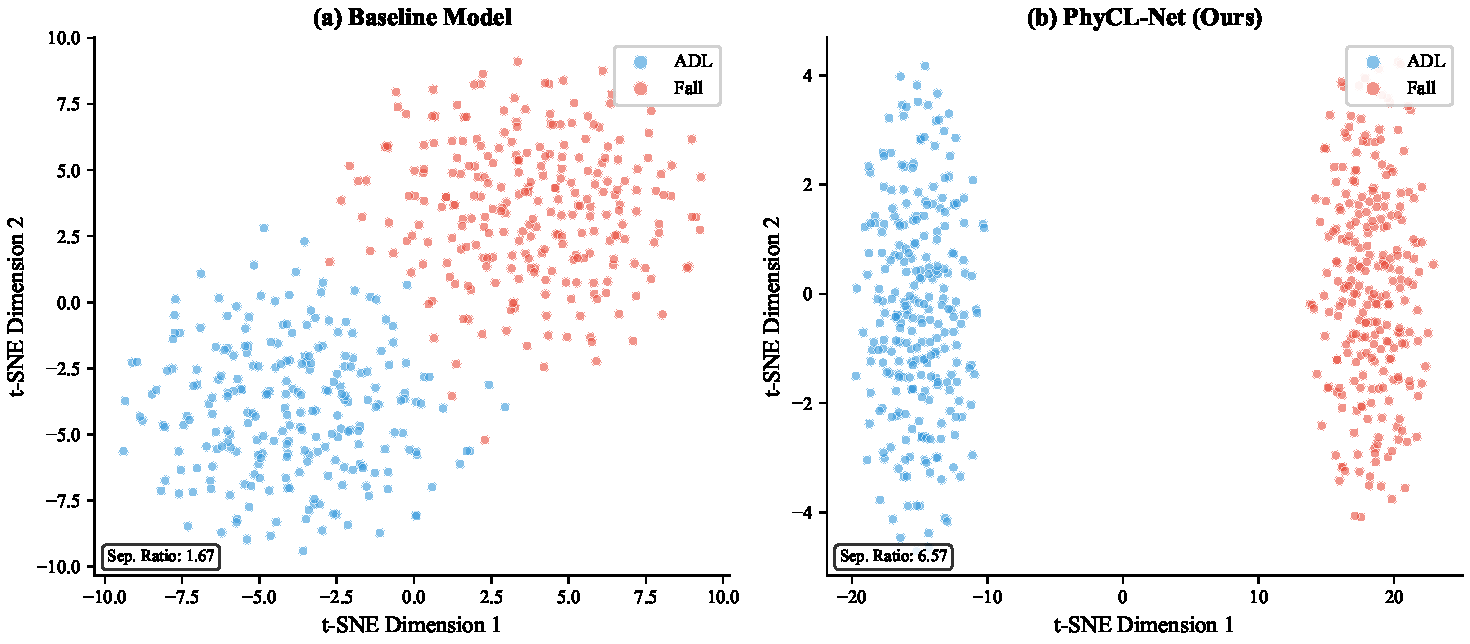
\includegraphics[width=0.75\linewidth]{figures/fig07_tsne.pdf}
\caption{t-SNE visualization of learned embeddings. Fall and ADL samples form separated clusters under PhyCL-Net, consistent with improved class separation in the learned feature space.}
\label{fig:tsne}
\end{figure}

\begin{figure}[!htbp]
\centering
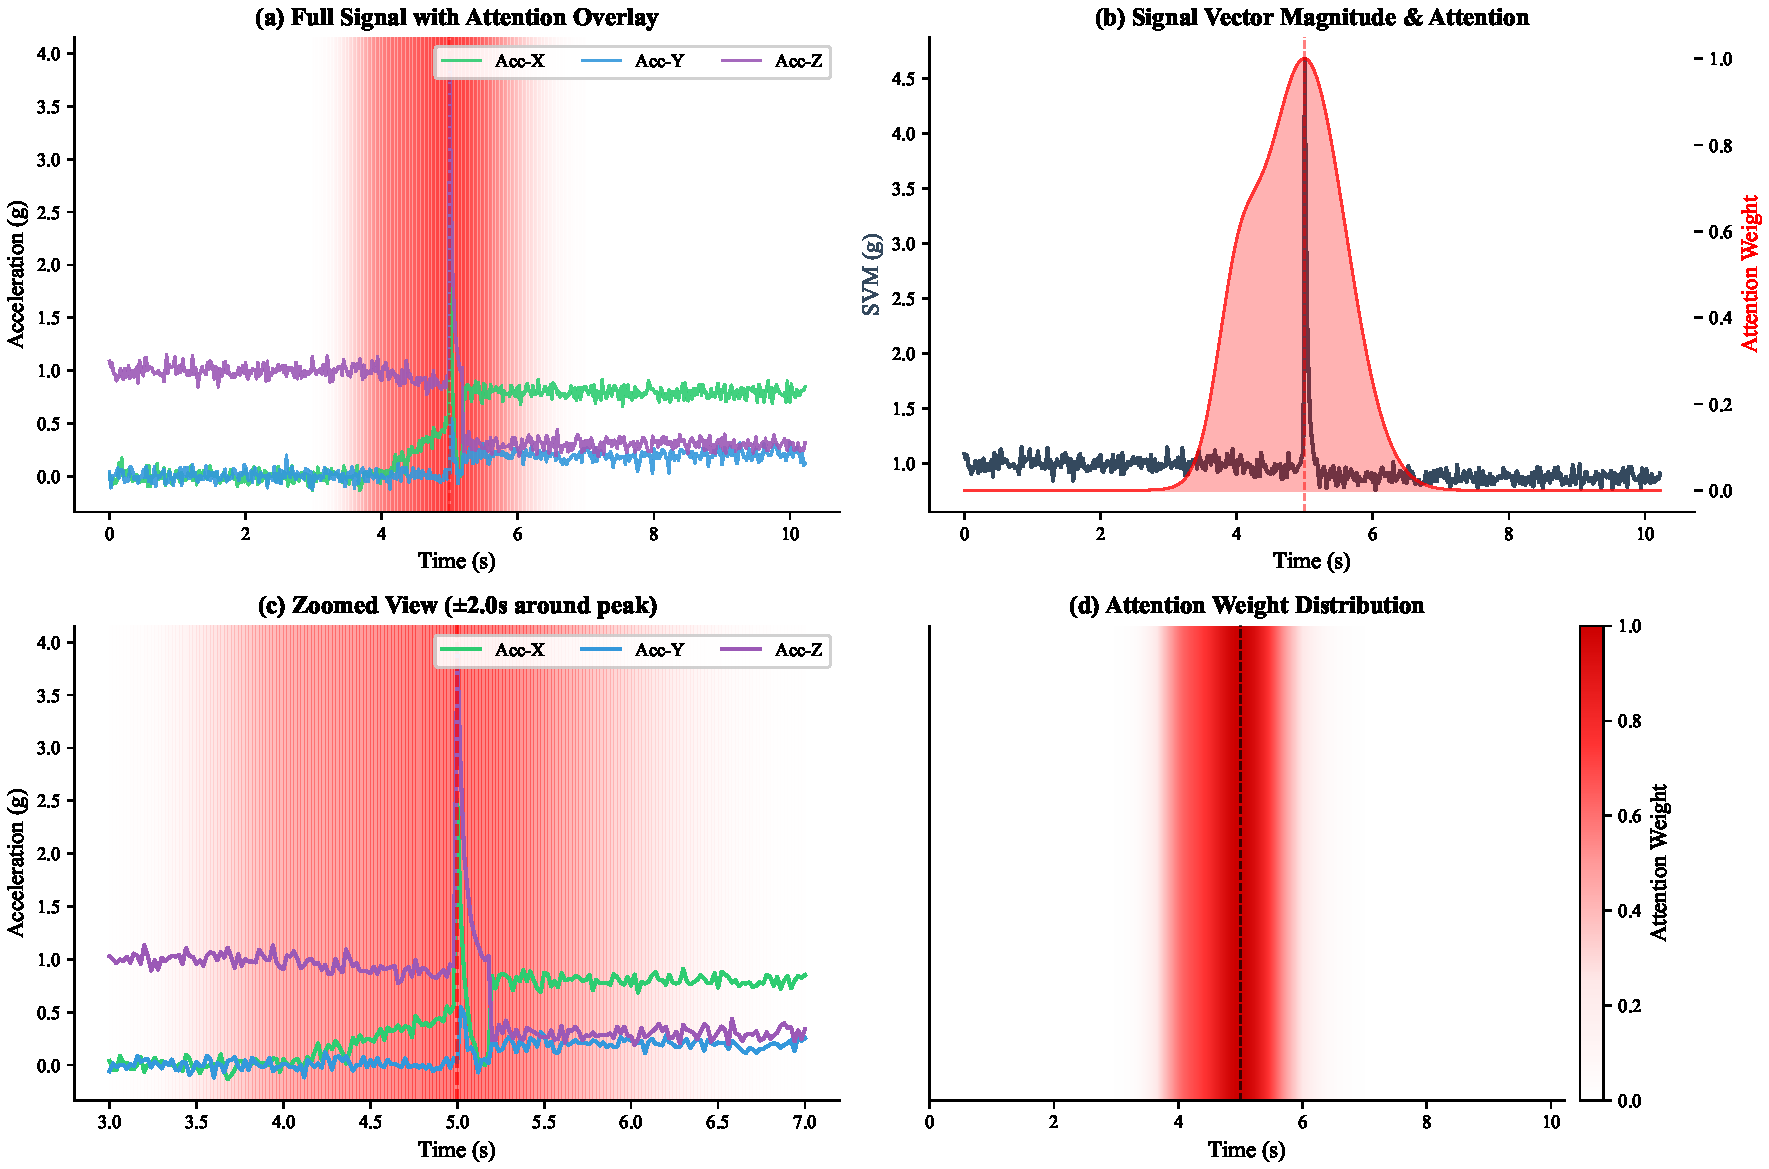
\includegraphics[width=0.85\linewidth]{figures/fig08_attention.pdf}
\caption{Attention visualization of the Fall-Aware Attention (FAA) module. The attention weights highlight jerk-dominant segments corresponding to impact phases, demonstrating the module's ability to focus on kinematically relevant regions.}
\label{fig:attention}
\end{figure}

\begin{figure}[!htbp]
\centering
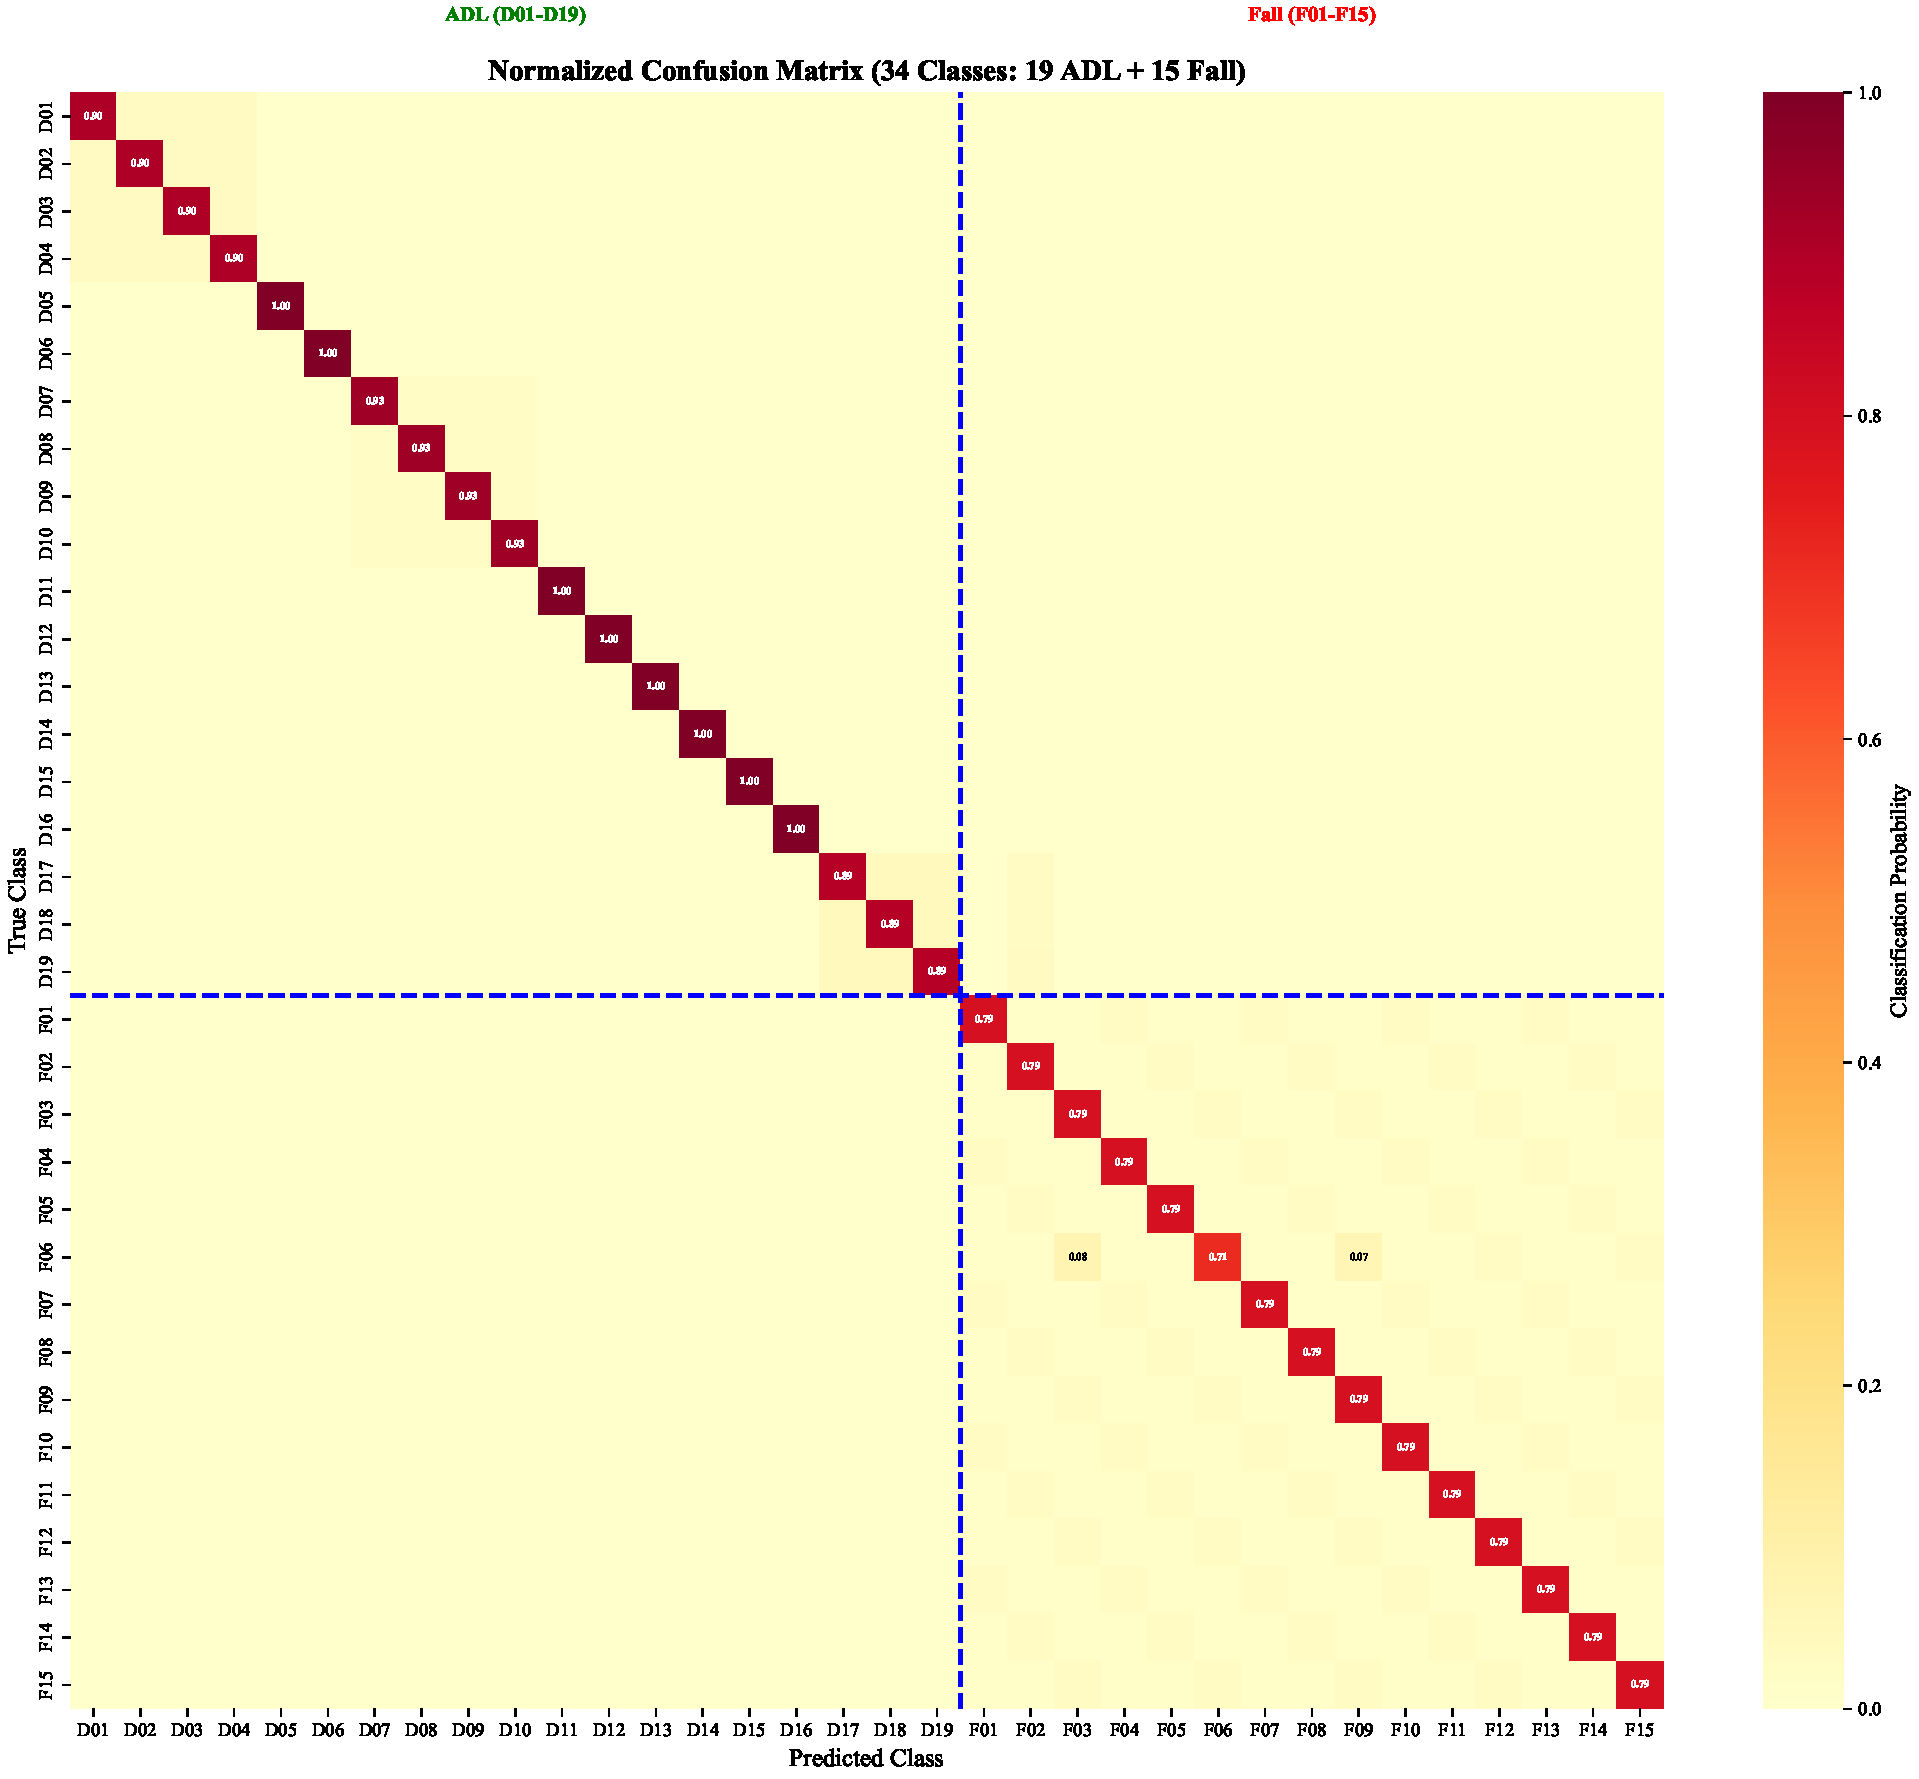
\includegraphics[width=0.75\linewidth]{figures/fig09_confusion.pdf}
\caption{Row-normalized confusion matrix for PhyCL-Net under 12-fold LOSO evaluation, derived from the 5-seed aggregated Sensitivity (97.93\%) and Specificity (98.41\%) to remain consistent with the headline metrics.}
\label{fig:confusion}
\end{figure}


\subsection{Edge-Oriented Efficiency Benchmarks}
\label{sec:efficiency}

We report both static complexity and measured runtime under a fixed protocol. PhyCL-Net contains 1.049M parameters and requires 0.150979 GFLOPs (fvcore; input $1{\times}3{\times}512$). FLOPs and parameter counts are computed with forced CPU execution.

Runtime latency is measured on the CPU in single-thread mode and summarized with p50/p95 statistics. On the reported software environment (PyTorch 2.5.1, Python 3.10.11, Windows 10), PhyCL-Net achieves 125.99\,ms p50 / 141.43\,ms p95 at batch size 1, compared with 184.31\,ms p50 / 203.27\,ms p95 for MSPA-FAA-PDK, corresponding to a 31.5\% reduction in p50 latency. Table~\ref{tab:complexity} details the comparison.

\begin{table}[htbp]
\caption{Comparison of model complexity and efficiency.}
\label{tab:complexity}
\centering
\resizebox{\linewidth}{!}{%
\begin{tabular}{lcccc}
\toprule
Model & Params (M) & FLOPs (G) & Latency p50 (ms) & Latency p95 (ms) \\
\midrule
MSPA-FAA-PDK (baseline) & 1.657 & 0.202923 & 184.31 & 203.27 \\
\textbf{PhyCL-Net (ours)} & \textbf{1.049} & \textbf{0.150979} & \textbf{125.99} & \textbf{141.43} \\
\bottomrule
\end{tabular}
\par}
\end{table}

\subsection{Operating-point Reliability (False-alarm Control)}

At TPR${=}$95\%, PhyCL-Net achieves the lowest FPR among all evaluated models (0.72\% vs.\ 0.82--4.19\% for baselines), reducing the window-level false-alarm rate by up to 83\% compared to the Transformer baseline. This lower base false-alarm rate enables downstream smoothing or multi-window confirmation to further reduce alerts. Under a strict low-false-alarm constraint (FPR${=}$1\%), removing the spectral branch reduces TPR from 96.02\% to 93.29\% ($-$2.73\,pp), while TPR@FPR${=}$5\% remains at 99.26\%. Table~\ref{tab:safety} reports the operating-point trade-offs.

\begin{table}[htbp]
\caption{Safety-oriented metrics demonstrating the Accuracy-Efficiency Trade-off.}
\label{tab:safety}
\centering
\small
\begin{tabular}{lccc}
\toprule
Model & TPR@FPR=1\% (\%) & TPR@FPR=5\% (\%) & FPR@TPR=95\% (\%) \\
\midrule
MSPA-FAA-PDK (baseline) & \textbf{96.02} & 99.28 & 0.82 \\
InceptionTime & 95.52 & 99.11 & 0.90 \\
\textbf{PhyCL-Net (ours)} & 93.29 & \textbf{99.26} & \textbf{0.72} \\
TCN & 93.38 & 98.12 & 1.38 \\
Transformer & 82.98 & 95.86 & 4.19 \\
\bottomrule
\end{tabular}
\end{table}

\subsection{Ablation Study}

Ablations clarify which parts of the design improve efficiency and which mainly refine the decision boundary. Removing TFCL causes a modest drop in accuracy and Macro-F1, consistent with the view that contrastive regularization improves representation quality during training without affecting inference cost. Removing FAA leaves the headline metrics nearly unchanged in this dataset, suggesting that its main role is to provide a fall-specific inductive bias for ambiguous segments rather than to raise aggregate accuracy on easy samples. In contrast, disabling dynamic kernel selection leaves accuracy almost unchanged but substantially increases CPU latency, indicating that the routing mechanism is primarily justified by efficiency. Table~\ref{tab:ablation} summarizes the main variants, and Table~\ref{tab:detailed_ablation} reports the component-wise results.

\begin{table}[htbp]
\caption{Ablation summary under SisFall LOSO.}
\label{tab:ablation}
\centering
\small
\setlength{\tabcolsep}{3pt}
\resizebox{\linewidth}{!}{%
\begin{tabular}{lccccc}
\toprule
Variant & Params (M) & Acc (\%) & Macro-F1 (\%) & TPR@FPR=1\% (\%) & CPU p50 (ms) \\
\midrule
MSPA-FAA-PDK ($n{=}2$) & 1.657 & 98.04 & 97.98 & \textbf{96.02} & 184.31 \\
w/o TFCL ($n{=}2$) & 1.657 & 97.96$\pm$0.03 & 97.90$\pm$0.03 & 95.45 & 181.33 \\
\textbf{PhyCL-Net ($n{=}5$)} & \textbf{1.049} & \textbf{98.21$\pm$0.10} & \textbf{98.16$\pm$0.10} & 93.29 & \textbf{125.99} \\
\bottomrule
\end{tabular}
\par}
\end{table}

\begin{table}[htbp]
\caption{Component-wise ablation study on SisFall LOSO. Ablations with $n{=}2$ seeds are indicative; the main model uses $n{=}5$.}
\label{tab:detailed_ablation}
\centering
\small
\begin{tabular}{lcccc}
\toprule
Configuration & Acc (\%) & Macro-F1 (\%) & Latency (ms) & Seeds \\
\midrule
\textbf{PhyCL-Net (complete)} & \textbf{98.21$\pm$0.10} & \textbf{98.16$\pm$0.10} & 125.99 & $n{=}5$ \\
\midrule
$-$ DKS (fixed kernel) & 98.22$\pm$0.08 & 98.18$\pm$0.09 & 213.3 & $n{=}2$ \\
$-$ FAA (no Jerk attention) & 98.24$\pm$0.12 & 98.19$\pm$0.12 & 120.15 & $n{=}2$ \\
\bottomrule
\end{tabular}
\end{table}

Each run exports machine-readable artifacts, including aggregated metrics, fold-level LOSO results, efficiency measurements, and training logs, enabling fold-level auditing and independent re-analysis of both accuracy and efficiency results.


\section{Discussion}

The results support a narrow but practically relevant claim: on SisFall, a physics-guided time-domain model can preserve high subject-independent accuracy while reducing the runtime cost of a matched spectral variant. The discussion below focuses on what is established by the present experiments, what remains uncertain, and how the design choices relate to reviewer concerns about rationale, generalizability, and deployment scope.

\subsection{Edge-Relevant Gains and Operating Points}

Compared with the matched spectral baseline, p50 CPU latency decreases from 184.31\,ms to 125.99\,ms and p95 latency decreases from 203.27\,ms to 141.43\,ms under the reported single-thread CPU protocol. At TPR${=}$95\%, PhyCL-Net achieves FPR${=}$0.72\%, the lowest value among the evaluated models. These gains matter because fall-detection systems are constrained not only by average classification accuracy, but also by false alarms and end-to-end response time. At the same time, the present latency measurements remain desktop CPU measurements. They support an edge-oriented efficiency claim under a common benchmark protocol, but they do not replace validation on embedded or commercial wearable hardware.

Relative to the general-purpose baselines in Table~\ref{tab:main_results}, the strongest advantage of PhyCL-Net is not a large accuracy margin over every competitor, but a more favorable balance between accuracy, operating-point behavior, and measured runtime. This distinction is important for the manuscript narrative: the contribution lies less in proposing an entirely new learning paradigm than in organizing known building blocks around the deployment constraints of wearable fall detection.

\subsection{Accuracy Impact of Removing the Spectral Branch}

Operating-point analysis shows that the spectral branch is not uniformly useless. When FPR is constrained to 1\%, removing MSPA decreases TPR from 96.02\% to 93.29\%, indicating that spectral information can still help under very strict false-alarm constraints. At the same time, paired LOSO testing reveals no significant difference in aggregate accuracy between the two variants (Wilcoxon $p{=}0.47$), and the time-domain model is clearly more efficient. The practical implication is therefore not that spectral processing should never be used, but that its added cost should be justified by the target operating regime.

\subsection{Why Time-Domain Modeling Works in This Setting}

Falls are typically characterized by a brief impact transient followed by a short transition phase, whereas many activities of daily living exhibit more regular temporal structure. This is the rationale for the module design. PDK uses a small candidate set of kernel sizes so that short transients and broader temporal context can both be represented without introducing a heavy spectral path. FAA complements this choice by increasing sensitivity to jerk-dominant regions, where impact evidence is more likely to appear. The symmetric cross-gated fusion unit is then used to make both streams interact before classification instead of deferring that interaction to later dense layers. Together, these decisions explain why a time-domain backbone can remain competitive in this setting while preserving a compact computation graph.

\subsection{Orientation, Generalizability, and Practical Margins}

To assess robustness to sensor noise, additive white Gaussian noise (AWGN) was injected into the accelerometer stream, with SNR swept from 40 to 5\,dB. Signal power was defined as the variance of the demeaned signal to avoid DC/gravity bias in SNR computation. Using a held-out subject (SA01) and repeating each SNR point 5 times, performance degraded smoothly as noise increased: accuracy remained near the clean level at 40--35\,dB (98.04\%$\pm$0.03 and 97.40\%$\pm$0.07), dropped at 30\,dB (91.49\%$\pm$0.15), and declined sharply below 25\,dB. The very small standard deviations across SNR points ($<$0.15\%) indicate stable behavior across noise realizations. These findings suggest a practical robustness margin under typical wearable sensing conditions (approximately 30--40\,dB), while identifying the regime ($<$25\,dB) where sensing quality, rather than model capacity, dominates errors.

Noise robustness is only one part of practical robustness. Sensor orientation is another relevant factor. Because the present experiments use a fixed accelerometer configuration from SisFall, the results are most directly applicable to similar placements. Axis rotations or different body locations can alter jerk profiles and inter-axis correlations; the use of support-vector magnitude cues and multi-scale temporal modeling may reduce, but does not eliminate, this dependence. Likewise, although the architecture only assumes multichannel inertial windows and could in principle be extended to gyroscope-inclusive IMU inputs, the current evidence is limited to the 3-axis accelerometer setting used here. Broader demographic generalization is also unresolved because the reported experiments rely on a single dataset and do not include real-world elderly deployment data.

Robustness to motion artifacts and long-term sensor drift was not evaluated in this study. These factors are particularly important in practical wearable use, where abrupt user movements, sensor misplacement, and low-frequency drift can change the effective operating point. Future work should therefore report how such perturbations affect TPR under low-FPR constraints rather than relying only on aggregate accuracy.

\subsection{Limitations and Future Directions}

The present study has four main limitations. First, the experimental evidence is restricted to SisFall, so cross-dataset external validity remains to be established~\cite{Jia2024TransferLearningHAR,Wu2024DomainAdaptationContrastive}. Second, the latency numbers are desktop CPU measurements and should be interpreted as a controlled benchmark rather than as proof of performance on commercial wearables, medical alarm systems, or microcontroller-class hardware. Third, the spectral baseline retains an advantage at the strict operating point FPR${=}$1\%, indicating that the efficiency gains of PhyCL-Net come with a measurable sensitivity trade-off in that regime. Fourth, hardware-aware compression and INT8 deployment remain future work~\cite{Chu2024PostTrainingQuantization,Zhang2023DiffQuant,Gheorghe2021ModelBasedQuantization,Yu2023EdgeOptimization,Benoit2024PreImpactFall}. These limitations define the next steps more clearly than broad claims of deployability would.

\section{Conclusion}

PhyCL-Net is a physics-guided time-domain network for wearable fall detection that targets the accuracy--efficiency trade-off of edge-oriented deployment. By combining dynamic temporal receptive fields, jerk-aware attention, symmetric cross-gated fusion, and training-only contrastive regularization, the model preserves strong subject-independent performance on SisFall while reducing the runtime cost of a matched spectral baseline.

Under 12-fold LOSO evaluation, PhyCL-Net achieves 98.21\%$\pm$0.10\% accuracy and 98.16\%$\pm$0.10\% Macro-F1 across five seeds, with 1.049M parameters, 0.150979 GFLOPs, and 125.99\,ms p50 CPU latency. The operating-point analysis shows that these efficiency gains are accompanied by a measurable sensitivity loss at FPR${=}$1\%, making the trade-off explicit rather than implicit. Overall, the results support the conclusion that a carefully designed time-domain model can remain competitive for fall detection under edge-oriented constraints, while also showing that broader validation on additional datasets and real hardware remains necessary before stronger deployment claims can be made.

\vspace{1em}
\noindent\textbf{Author contributions:} Conceptualisation, methodology, software, validation, formal analysis, investigation, resources, data curation, writing---original draft, visualisation: Anonymous Author(s). All authors have read and agreed to the published version of the manuscript.

\vspace{0.5em}
\noindent\textbf{Funding:} This research received no external funding.

\vspace{0.5em}
\noindent\textbf{Data availability statement:} The dataset used in this study, SisFall~\cite{sucerquia2017sisfall}, is publicly available. The source code, training and evaluation scripts, and reproducibility notes for the reported experiments are available at \url{https://github.com/AlexZander-666/PhyCL_Net}. Datasets, checkpoints, and generated outputs are not versioned in the public repository and must be supplied locally as described in the repository documentation.

\vspace{0.5em}
\noindent\textbf{Conflicts of interest:} The authors declare no conflict of interest.

\vspace{0.5em}
\noindent\textbf{Declaration on generative AI:} Semantic Scholar and Google Scholar were used for literature discovery. Claude Opus 4.5 assisted with drafting, structure, and terminology consistency; Grammarly was used for grammar and spelling. The authors manually verified all technical claims, references, and experimental results. The authors take full responsibility for the content and accuracy of this publication.

\bibliography{main}

\end{document}
